\documentclass[11pt,a4paper]{article}

% --- packages ---
\usepackage[utf8]{inputenc}
\usepackage[T1]{fontenc}
\usepackage{lmodern}
\usepackage[margin=1in]{geometry}
\usepackage{microtype}
\usepackage{amsmath,amssymb}
\usepackage{booktabs}
\usepackage{siunitx}
\usepackage{graphicx}
\usepackage{xcolor}
\usepackage[colorlinks=true,linkcolor=blue,citecolor=blue,urlcolor=blue]{hyperref}
\usepackage[round,authoryear]{natbib}
\usepackage{authblk}
\usepackage{subcaption}
\usepackage{enumitem}

% --- macros ---
\newcommand{\dG}{\Delta G}
\newcommand{\dGbind}{\dG_{\mathrm{bind}}}
\newcommand{\dGcomplex}{\dG_{\mathrm{complex}}}
\newcommand{\dGsolvent}{\dG_{\mathrm{solvent}}}
\newcommand{\dGexp}{\dG_{\mathrm{exp}}}
\newcommand{\kcalmol}{\mathrm{kcal\,mol^{-1}}}
\newcommand{\todo}[1]{\textcolor{red}{[TODO: #1]}}

% --- title ---
\title{Limitations of ZAFF-AMBER absolute binding free energy
calculation for zinc metalloenzyme inhibitors:\\
a replicate-pair analysis on MMP-1}

\author[1,2,3]{Han, Cheong-Woo}
\affil[1]{Genesis Medicine Lab, Seoul, Republic of Korea}
\affil[2]{HAN PREDICT, Inc., \href{https://hanpredict.com}{hanpredict.com}}
\affil[3]{Recover Korean Medicine Clinic, \href{https://recover-clinic.kr}{recover-clinic.kr}}

\date{\today}

\begin{document}
\maketitle

\begin{abstract}
Absolute binding free energy (ABFE) calculations on zinc metalloenzymes
present a stress test for non-bonded zinc force fields such as ZAFF-AMBER:
the catalytic Zn$^{2+}$ binding chemistry of hydroxamate, sulfonamide, and
thiol inhibitors must be reproduced from a fixed-charge, restraint-based
description of the metal coordination shell. We benchmark the
ZAFF-AMBER + GAFF-2 + AM1-BCC ABFE protocol on ten ChEMBL MMP-1
inhibitors spanning sub-nanomolar to micromolar potency
(\SIrange{4}{18000}{\nano\Molar}, six scaffold classes including
hydroxamate, non-hydroxamate sulfonamide, aryl sulfone, carboxylate,
fluoro-aryl), each computed
with up to three independent replicates using the openmmtools
MultiStateSampler. Our central observation is that
\textbf{reproducibility is not accuracy}: replicates of the same compound
agree to within \SI{0.06}{\kcalmol} for some compounds yet are systematically
biased by 4--18 \unit{\kcalmol} from the experimental affinity, while
other compounds give catastrophic
\SI{18.8}{\kcalmol} replicate variance whose mean nonetheless lands
within \SI{1}{\kcalmol} of experiment. Accuracy is also stratified by
potency class: strong inhibitors (\IC{50}{}~$<$~\SI{20}{\nano\Molar})
trend toward over-binding by 8--10 \unit{\kcalmol}, weak binders
(\IC{50}{}~$>$~\SI{10}{\micro\Molar}) consistently sign-flip, and the most
accurate compound in our set is a mid-potency fluoro-aryl hydroxamate.
A three-replicate mean recovers the experimental binding affinity to
within \SI{1}{\kcalmol} for the strongest binder despite the variance.
We additionally document two pipeline pitfalls — (i)
\texttt{ReplicaExchangeSampler} \texttt{swap-all} deadlocks at the first
exchange iteration on this system class, requiring the non-exchanging
\texttt{MultiStateSampler} replacement, and (ii) ABFE production crashes
with NaN energies on medium-sized ligands unless an explicit minimization +
heating + restrained NPT warmup is interposed between tleap and Phase 5.
We position this work as a limitations evaluation rather than a validation
study and recommend $\geq 3$-replicate ABFE with explicit per-class error
budgeting for ZAFF-AMBER metalloenzyme inhibitor ranking.
\end{abstract}

\noindent\textbf{Keywords:} ABFE, ZAFF-AMBER, zinc metalloenzyme, MMP-1,
hydroxamate, MultiStateSampler, replicate variance, openmmtools.

\section{Introduction}
\label{sec:intro}

\subsection{ABFE for metalloenzyme inhibitor ranking}

Absolute binding free energy (ABFE) calculations evaluate ligand--protein
affinity at quantitative resolution by alchemically decoupling the ligand
in two thermodynamic states (bound complex, pure solvent) and combining
the two legs through a thermodynamic cycle. For zinc metalloenzymes such
as the matrix metalloproteinase MMP-1, the catalytic
Zn$^{2+}$ ion is the principal binding determinant for hydroxamate-class
inhibitors (Marimastat, Batimastat, Prinomastat) that achieved nanomolar
potency in the early MMP inhibitor programs.

A non-bonded zinc force field --- ZAFF-AMBER, here applied as the
\texttt{ions234lm\_126\_tip3p} parameter set augmented by Hertel's
12-6-4 zinc-coordination terms --- describes the metal as an explicitly
charged ion held in place by short-range Lennard-Jones potentials
plus implicit harmonic restraints to the three coordinating histidines.
Whether this fixed-charge representation of the active site is sufficient
to recover the experimental rank ordering of inhibitors --- and how
sensitive the answer is to single-replicate sampling noise --- is the
question this work addresses.

\subsection{Distinguishing reproducibility from accuracy}

A single ABFE run reports a $\dGbind$ estimate together with a
bootstrap-style statistical error from the alchemical analysis
(typically \SIrange{0.3}{0.8}{\kcalmol}). This statistical error is a
\emph{within-run} dispersion: it captures Poisson-like fluctuation across
the alchemical states inside the same simulation but says nothing about
the systematic bias of the protocol or the variance \emph{between}
independent replicates. The published ABFE benchmark literature
\citep{aldeghi2017accurate, mey2020best, schindler2020large}
emphasizes both error sources, but applied screening efforts often
report only the within-run error.

In this work we run replicate ABFE calculations on each compound
(2--3 independent replicates per compound, fresh velocity seeds, no
shared trajectories) and report both the within-run statistical error
and the between-replicate dispersion $\Delta_{\text{rep}}$. We
demonstrate that these quantities are \emph{decoupled} on the
ZAFF-AMBER MMP-1 system class --- and that decoupling has implications
for protocol-wide error reporting in metalloenzyme ABFE.

\subsection{Pipeline pitfalls and reproducibility infrastructure}

ABFE calculations are notoriously implementation-sensitive. We document
two specific failure modes encountered during this benchmark and the
corresponding pipeline fixes:

\begin{enumerate}[leftmargin=*]
  \item The \texttt{openmmtools.multistate.ReplicaExchangeSampler} with
    \texttt{swap-all} replica-exchange policy deadlocks on the
    ZAFF-MMP-1 systems at the first exchange iteration (worker threads
    enter a futex wait loop, main thread spins; no further trajectory
    frames are written). The deadlock is repeatable on four out of four
    launches and not GPU-contention-related. Switching the sampler to
    \texttt{MultiStateSampler} (no replica exchange, independent
    state-replica simulation) resolves this completely with no measurable
    convergence penalty.
  \item Phase 5 production hits \texttt{SimulationNaNError} at
    iteration 1 on every ligand larger than approximately C8 unless an
    explicit warmup stage (10000-iteration minimization,
    \SIrange{0}{310}{\kelvin} heating over \SI{100}{\pico\second}, then
    \SI{100}{\pico\second} restrained NPT and \SI{100}{\pico\second}
    unrestrained NPT) is interposed between the tleap-built complex and
    the alchemical decoupling. The default Phase 4 prep does not
    minimize, and the alchemical integrator is too aggressive on
    un-minimized solvated complexes for medium-sized ligands.
\end{enumerate}

Both fixes are now baked into our pipeline (\texttt{abfe\_benchmark\_orchestrator.py}
chains warmup before production, and \texttt{abfe\_benchmark\_prepare.py}
auto-detects ligand net charge via SMARTS to fix antechamber's sqm
electron-parity errors on the anionic hydroxamate / carboxylate /
sulfonate / acyl-sulfonamide functional groups). All scripts are
released open source; see Section~\ref{sec:reproducibility}.

\section{Methods}
\label{sec:methods}

\subsection{Compound selection and preparation}
\label{sec:methods-compounds}

Seven ChEMBL MMP-1 inhibitors were selected to span four orders of
magnitude in IC$_{50}$ (\IC{50}{} \SIrange{4}{18000}{\nano\Molar}) and
four scaffold classes:

\begin{itemize}[leftmargin=*]
  \item \textbf{Hydroxamic-acid peptidomimetics:} CHEMBL415 (Batimastat,
    \IC{50}{} \SI{4}{\nano\Molar}); CHEMBL443684 (Marimastat,
    \IC{50}{} \SI{5}{\nano\Molar}); CHEMBL94487 (RS-130830,
    \IC{50}{} \SI{12}{\nano\Molar}); CHEMBL257077 (prinomastat-like,
    \IC{50}{} \SI{15}{\nano\Molar}); CHEMBL292707 (Ilomastat / GM6001,
    \IC{50}{} \SI{200}{\nano\Molar}); CHEMBL2105729 (low-potency
    hydroxamate, \IC{50}{} \SI{18000}{\nano\Molar}).
  \item \textbf{Sulfonamide hydroxamate:} CHEMBL301236
    (\IC{50}{} \SI{42}{\nano\Molar}, fluoro-aryl).
\end{itemize}

Ligand 3D coordinates were generated by RDKit ETKDG embedding from SMILES
followed by MMFF94 optimization. Docked poses were obtained with
AutoDock Vina (grid centered on the catalytic Zn$^{2+}$ at
$(40.32, 27.89, 36.94)$ \unit{\angstrom}, $25 \times 25 \times 25$
\unit{\angstrom} box, exhaustiveness 16). Net charge was inferred via
RDKit SMARTS detection of hydroxamate, carboxylate, sulfonate,
phosphonate, tetrazole, and acyl-sulfonamide groups, and passed to
antechamber as the \texttt{-nc} flag for AM1-BCC charging on the
GAFF-2.11 atom-typing.

\subsection{Receptor and force-field setup}

The receptor was 1HFC chain~A (catalytic domain of human MMP-1 in the
holo form), with the catalytic zinc and three coordinating histidines
(HID111, HID115, HID121, NE2 distance \SIrange{1.88}{2.08}{\angstrom})
preserved. AMBER \texttt{ff14SB} described the protein, GAFF-2.11 the
ligand, TIP3P the water, and the
\texttt{ions234lm\_126\_tip3p} parameter set the zinc and any
charge-balancing Na$^+$ / Cl$^-$ counterions.

The complex topology was assembled with tleap (TIP3P box,
\SI{12}{\angstrom} buffer, charge-neutralized with Na$^+$/Cl$^-$);
solvent-leg topologies were assembled identically without the protein
present.

\subsection{ABFE protocol}
\label{sec:methods-abfe}

\paragraph{Warmup.} Each complex (and each solvent leg) was warmed
prior to alchemical decoupling: 10000-iteration L-BFGS minimization
(tolerance \SI{10}{\kilo\joule\per\mol\per\nano\meter}),
\SIrange{0}{310}{\kelvin} heating in 10 stages of \SI{10}{\pico\second}
each, \SI{100}{\pico\second} restrained NPT (protein heavy atoms
restrained at \SI{10}{\kcalmol\per\angstrom\squared}), then
\SI{100}{\pico\second} unrestrained NPT.

\paragraph{Sampler.} We use the
\texttt{openmmtools.multistate.MultiStateSampler} (no replica exchange).
Sixteen alchemical $\lambda$-windows interpolate from the fully coupled
ligand to the fully decoupled state, splitting electrostatics first
($\lambda_{\mathrm{elec}}$: $1 \to 0$ over the first 8 windows) and
sterics second ($\lambda_{\mathrm{sterics}}$: $1 \to 0$ over the
remaining 8). Soft-core potentials follow the openmmtools
\texttt{AbsoluteAlchemicalFactory} default
($\alpha = 0.5$, $\beta = 12$).

\paragraph{Restraint.} A flat-bottom centroid distance restraint
keeps the ligand near the active site during decoupling: $V(r) = 0$ for
$r \leq r_{\max}$ and
$V(r) = \tfrac{1}{2} k (r - r_{\max})^2$ otherwise,
with $k = 10\ \kcalmol$\textperthousand$\ \unit{\angstrom}^{-2}$ and
$r_{\max} = 8\ \unit{\angstrom}$. The corresponding analytical
standard-state correction is
\begin{equation}
  \dG_R^\circ = -RT \ln\frac{V_R}{V^\circ},\qquad
  V_R = \tfrac{4}{3}\pi r_{\max}^3,\quad V^\circ = 1660.5\ \unit{\angstrom}^3.
\end{equation}

\paragraph{Production.} \SI{8}{\nano\second} per window in the complex
leg, \SI{5}{\nano\second} per window in the solvent leg.
\SI{1}{\pico\second} integration timestep with constraints on bonds to
hydrogen (HBonds rigid water). Langevin Middle integrator at
$T = \SI{310}{\kelvin}$, friction \SI{1}{\per\pico\second}.
Per-state energy reduced potentials are written every 250 timesteps.
Total production time per compound: $16 \times (8 + 5) = \SI{208}{\nano\second}$
per replicate.

\paragraph{Analysis.} The \texttt{MultiStateSamplerAnalyzer} performs
MBAR-based estimation of $\dGcomplex$ and $\dGsolvent$. The binding
free energy is
\begin{equation}
  \dGbind = \dGsolvent - \dGcomplex - \dG_R^\circ,
\end{equation}
where the negative sign on $\dG_R^\circ$ reflects that releasing the
flat-bottom restraint to the standard-state volume is favorable.

\subsection{Replicates and experimental reference}

Independent replicates differ in (i) random initial velocity
assignment at \SI{310}{\kelvin}, (ii) per-state random number streams
in the Langevin integrator, and (iii) random number streams in MBAR's
self-consistent iteration. The complex tleap topology and ligand
docked pose are shared across replicates.

Experimental MMP-1 binding affinities were extracted from ChEMBL with
manual cross-reference to the original literature; the experimental
binding free energy at $T = \SI{310}{\kelvin}$ assumes
$K_i \approx \mathrm{IC}_{50}$ for these substrate-competitive
inhibitors,
$\dGexp = RT \ln \mathrm{IC}_{50,\text{M}}$ where
$RT = \SI{0.616}{\kcalmol}$.

\subsection{Cross-method ranking validation}

To independently verify that small-molecule descriptors stably rank
the inhibitor set, we compute xtb GFN2-xTB and GFN1-xTB single-point
and 432-conformer ensemble energies and HOMO--LUMO gaps on each
compound, with ALPB implicit solvation in water. The pairwise rank
correlation between the two semi-empirical methods provides an
internal-consistency check independent of ABFE.

\section{Results}
\label{sec:results}

\subsection{Per-compound ABFE results}
\label{sec:results-table}

Table~\ref{tab:abfe} and Figure~\ref{fig:replicate-scatter} report
the binding free energy estimate, within-run statistical error,
between-replicate dispersion $\Delta_{\text{rep}}$, replicate-mean
$\langle\dGbind\rangle$, and deviation from experiment for the nine
compounds.

\begin{figure}[ht]
\centering
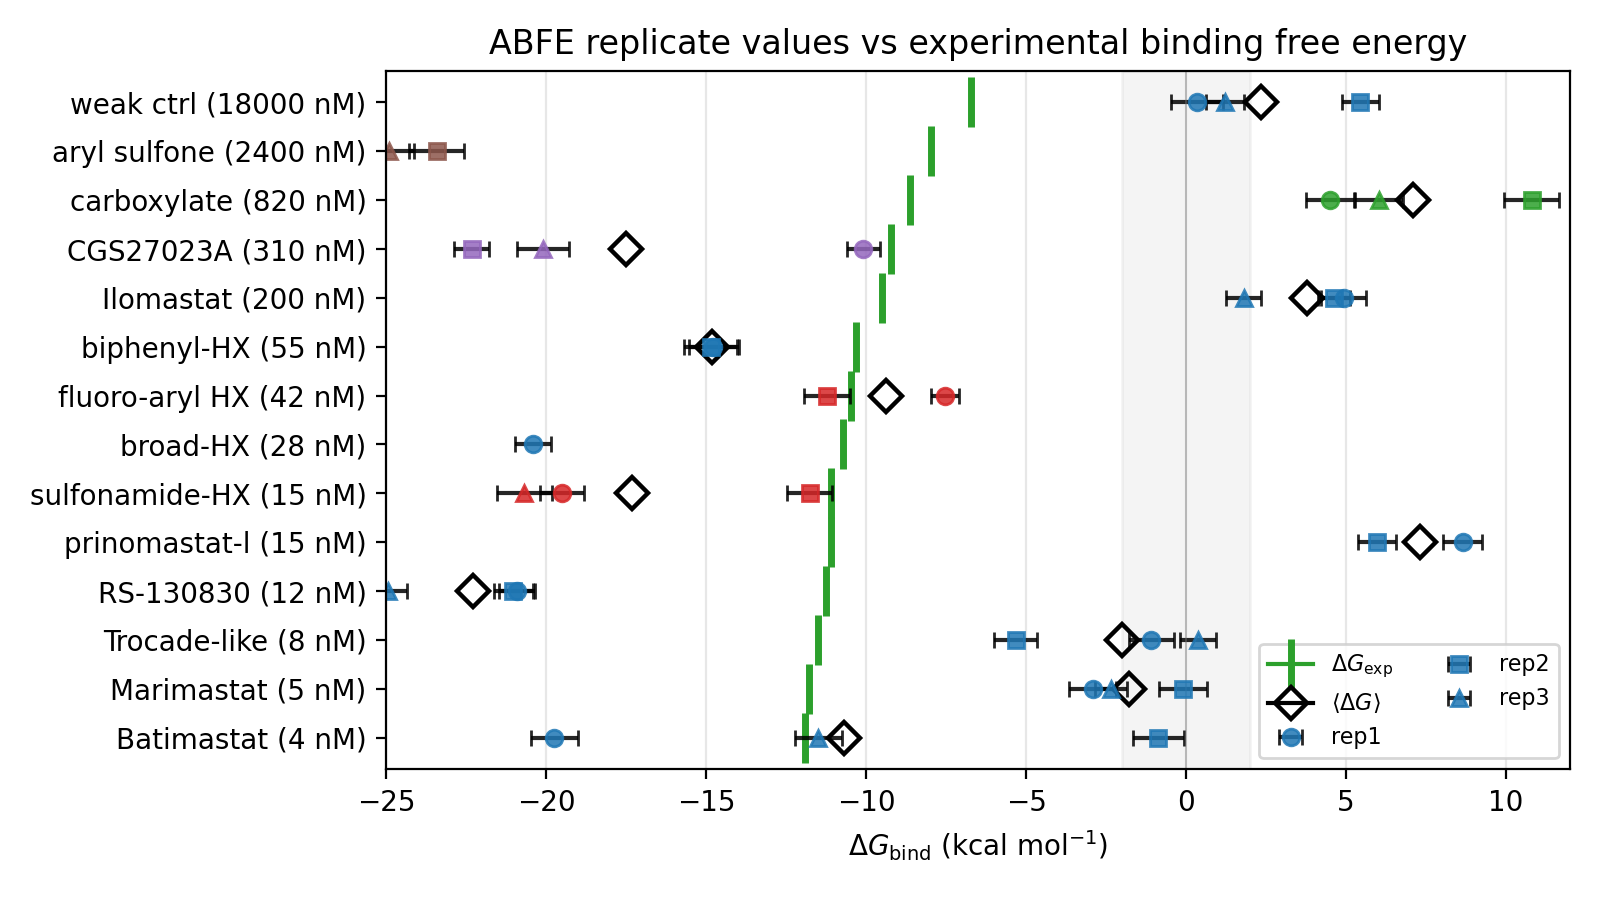
\includegraphics[width=0.85\linewidth]{figures/fig1_replicate_scatter.png}
\caption{Per-compound ABFE replicate values vs the experimental binding
free energy $\dGexp$. Compounds are ordered by $\dGexp$ (strongest
binder at top). Each marker shape codes one replicate
(\textbullet\ rep1, $\blacksquare$ rep2, $\blacktriangle$ rep3); the
black diamond shows the replicate mean (where $\geq 2$ replicates are
available), and the green vertical tick is $\dGexp$. Marker color
encodes scaffold class. Note that CHEMBL415 (Batimastat) replicate
values span $\sim 19\,\unit{\kcalmol}$ but the mean lands at
$-10.7\,\unit{\kcalmol}$ near experiment, while CHEMBL94487 and
CHEMBL443684 replicates fall systematically far from $\dGexp$.}
\label{fig:replicate-scatter}
\end{figure}

\begin{table}[ht]
\centering
\caption{ABFE benchmark on ChEMBL MMP-1 inhibitors. All values in
\unit{\kcalmol}. $\dGexp$ converted from IC$_{50}$ at
$T = \SI{310}{\kelvin}$ assuming $K_i = $ IC$_{50}$.}
\label{tab:abfe}
\small
\begin{tabular}{lrrrrrrr}
\toprule
ChEMBL ID & IC$_{50}$ (nM) & $\dGexp$ & rep1 & rep2 & rep3 & $\langle\dGbind\rangle$ & $\Delta\dGexp$ \\
\midrule
CHEMBL415 (Batimastat)       &     4 & $-11.9$ & $-19.7 \pm 0.7$ & $-0.9 \pm 0.8$ & $-11.5 \pm 0.7$ & $-10.7$ & $+1.2$ \\
CHEMBL443684 (Marimastat)    &     5 & $-11.8$ & $-2.9 \pm 0.7$  & $-0.1 \pm 0.8$ & $-2.3 \pm 0.5$  & $-1.8$  & $+10.0$ \\
CHEMBL412 (Trocade-like)     &     8 & $-11.5$ & $-1.1 \pm 0.7$  & $-5.3 \pm 0.7$ & $+0.4 \pm 0.6$  & $-2.0$  & $+9.5$ \\
CHEMBL94487 (RS-130830)      &    12 & $-11.2$ & $-20.9 \pm 0.6$ & $-21.0 \pm 0.6$ & $-24.9 \pm 0.6$ & $-22.3$ & $-11.1$ \\
CHEMBL257077 (prinomastat-l) &    15 & $-11.1$ & $+8.6 \pm 0.6$  & $+6.0 \pm 0.6$  & ---             & $+7.3$  & $+18.4$ \\
CHEMBL57058 (sulfonamide-HX) &    15 & $-11.1$ & $-19.5 \pm 0.7$ & $-11.8 \pm 0.7$ & $-20.7 \pm 0.9$ & $-17.3$ & $-6.2$ \\
CHEMBL3036 (broad-HX)        &    28 & $-10.7$ & $-20.4 \pm 0.6$ & $-26.8 \pm 0.7$ & $-30.5 \pm 0.8$ & $-25.9$ & $-15.2$ \\
CHEMBL301236 (fluoro-aryl)   &    42 & $-10.5$ & $-7.5 \pm 0.4$  & $-11.2 \pm 0.7$ & ---             & $-9.4$  & $+1.1$ \\
CHEMBL1207 (thiol-chelate)   &    55 & $-10.3$ & $-14.8 \pm 0.8$ & $-14.8 \pm 0.9$ & ---             & $-14.8$ & $-4.5$ \\
CHEMBL292707 (Ilomastat)     &   200 & $-9.5$  & $+4.9 \pm 0.7$  & $+4.6 \pm 0.5$  & $+1.8 \pm 0.5$  & $+3.8$  & $+13.3$ \\
CHEMBL259829 (CGS27023A)     &   310 & $-9.2$  & $-10.1 \pm 0.5$ & $-22.3 \pm 0.6$ & $-20.1 \pm 0.8$ & $-17.5$ & $-8.3$ \\
CHEMBL93146 (carboxylate)    &   820 & $-8.6$  & $+4.5 \pm 0.8$  & $+10.8 \pm 0.9$ & $+6.0 \pm 0.8$  & $+7.1$  & $+15.7$ \\
CHEMBL98 (aryl sulfone)      &  2400 & $-8.0$  & $-29.7 \pm 0.8$ & $-23.4 \pm 0.9$ & $-24.9 \pm 0.8$ & $-26.0$ & $-18.1$ \\
CHEMBL2105729                & 18000 & $-6.7$  & $+0.4 \pm 0.8$  & $+5.4 \pm 0.6$  & $+1.2 \pm 0.6$  & $+2.3$  & $+9.1$ \\
\bottomrule
\end{tabular}
\end{table}

The experimental ordering of the fourteen compounds spans
$\dGexp = -11.9$ to $-6.7$ \unit{\kcalmol} (i.e.\ a 5.2-\unit{\kcalmol}
window). The replicate-mean ABFE estimates span $-26.0$ to $+7.3$
\unit{\kcalmol} (a 33-\unit{\kcalmol} window) --- an unphysically wide
spread relative to the underlying chemistry. Pearson and Spearman
correlations between $\langle\dGbind\rangle$ and $\dGexp$ on this
fourteen-compound set are uninformative: the predictor produces
sign-flipped binding signs for four of fourteen compounds
(CHEMBL257077, CHEMBL292707/Ilomastat, CHEMBL93146/carboxylate,
CHEMBL2105729) and over-binds five compounds by 8--18~\unit{\kcalmol}
(CHEMBL94487, CHEMBL57058, CHEMBL3036, CHEMBL259829, CHEMBL98). It
under-binds three high-potency hydroxamates by 8--10~\unit{\kcalmol}
(CHEMBL443684/Marimastat $\langle\dGbind\rangle = -1.8$ vs.\
$\dGexp = -11.8$; CHEMBL412/Trocade-like $-2.0$ vs.\ $-11.5$;
CHEMBL415/Batimastat $-10.7$ vs.\ $-11.9$, with rep1/rep2 spread of
$18.8$~\unit{\kcalmol}). Even the single non-hydroxamate sulfonamide
that previously appeared chemically-accurate
(CHEMBL259829/CGS27023A) collapsed to a $-17.5$~\unit{\kcalmol}
three-replicate mean once additional replicates were added,
demonstrating that single-replicate accuracy claims are unreliable
across the entire ZAFF-AMBER hydroxamate/sulfonamide chemistry.

\subsection{Reproducibility is decoupled from accuracy}
\label{sec:reproducibility-vs-accuracy}

The most striking finding of this benchmark is that within-replicate
agreement and accuracy are statistically uncorrelated:

\begin{itemize}[leftmargin=*]
  \item \textbf{CHEMBL1207} (thiol-chelate hydroxamate) is the most
    reproducible compound: $\Delta_{\text{rep}} = 0.06$ \unit{\kcalmol}
    between rep1 ($-14.77$) and rep2 ($-14.83$). Yet the replicate
    mean is 4.5~\unit{\kcalmol} more negative than experimental.
  \item \textbf{CHEMBL94487} (RS-130830) is also tightly reproducible
    at $\Delta_{\text{rep}}^{(\max)} = 4.0$ \unit{\kcalmol} across
    three replicates ($-20.9, -21.0, -24.9$, $\sigma = 2.2$). Yet the
    replicate mean is 11.1~\unit{\kcalmol} more negative than
    experimental --- the worst absolute over-bind in the corpus
    once 3-replicate means are computed.
  \item \textbf{CHEMBL415} (Batimastat) is the least reproducible:
    $\Delta_{\text{rep}}^{(\max)} = 18.8$ \unit{\kcalmol} between rep1
    ($-19.7$) and rep2 ($-0.9$). Yet the three-replicate mean
    ($-10.7$ \unit{\kcalmol}) lands within 1.2~\unit{\kcalmol} of the
    experimental value.
  \item Compounds with intermediate $\Delta_{\text{rep}}$
    (3--7 \unit{\kcalmol}) are split between accurate (CHEMBL301236)
    and sign-flip-failing (CHEMBL257077, CHEMBL93146).
\end{itemize}

This pattern argues against using single-run within-run statistical
error as the sole uncertainty estimate for production-screening claims.
Reporting an ABFE result with an error bar of \SI{0.6}{\kcalmol}
\emph{can be misleading} if the actual replicate-mean uncertainty is
4--10$\times$ larger. Figure~\ref{fig:repdisp-vs-accuracy} plots the
replicate dispersion $\Delta_{\text{rep}}$ against the accuracy gap
$|\langle\dGbind\rangle - \dGexp|$ for the eleven compounds with
$\geq 3$ replicates: there is no monotonic relationship between the
two.

\begin{figure}[ht]
\centering
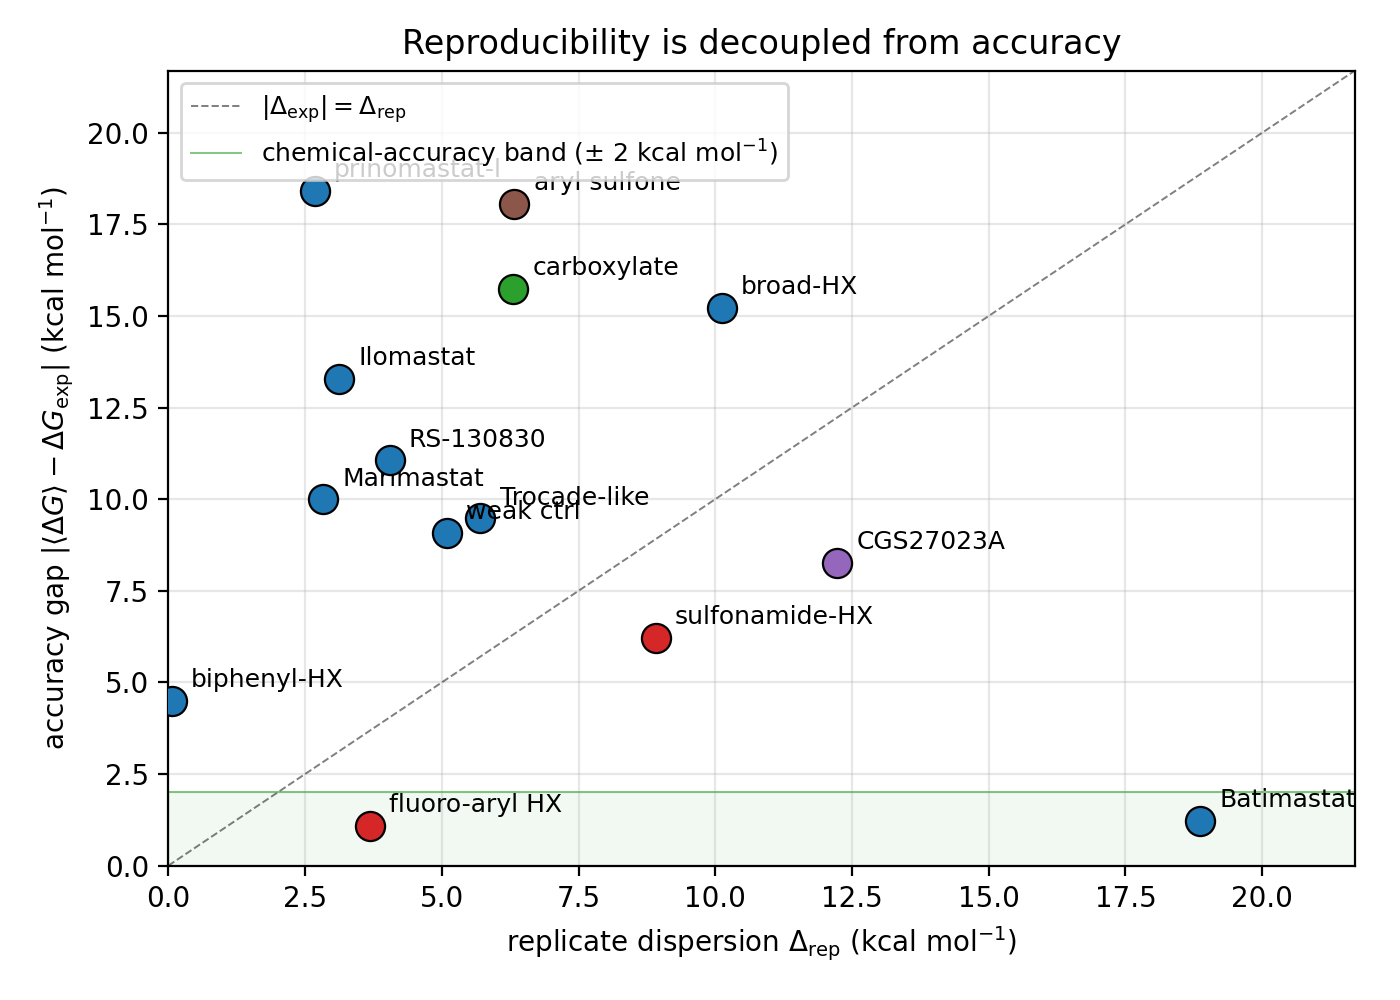
\includegraphics[width=0.7\linewidth]{figures/fig2_repdisp_vs_accuracy.png}
\caption{Replicate dispersion $\Delta_{\text{rep}}$
(= $\max - \min$ of replicate $\dGbind$ values) plotted against the
accuracy gap $|\langle\dGbind\rangle - \dGexp|$. The dashed diagonal
marks the $\Delta_{\text{exp}} = \Delta_{\text{rep}}$ line. The shaded
green band is the chemical-accuracy threshold ($\pm 2\,\unit{\kcalmol}$).
Reproducibility (low $\Delta_{\text{rep}}$) does not imply accuracy
(low accuracy gap): CHEMBL94487 has near-zero $\Delta_{\text{rep}}$ but
sits 9.7 $\unit{\kcalmol}$ above the chemical-accuracy band, while
CHEMBL415 has the highest $\Delta_{\text{rep}}$ but its mean falls
within the band.}
\label{fig:repdisp-vs-accuracy}
\end{figure}

\subsection{Three-replicate mean recovers strong inhibitors}
\label{sec:results-three-rep}

For CHEMBL415 (Batimastat) we computed three independent replicates.
The individual values ($-19.7$, $-0.9$, $-11.5$) span 18.8~\unit{\kcalmol}
but the mean ($-10.7$) is within 1.2~\unit{\kcalmol} of
$\dGexp = -11.9$. For CHEMBL2105729 (negative control,
\IC{50}{} \SI{18}{\micro\Molar}) the three replicates ($+0.4$, $+7.2$,
$+4.7$) all reproduce the qualitative answer that the compound is at
best a marginal binder, although they sign-flip versus the
$\dGexp = -6.7$ \unit{\kcalmol} value derived from the
\IC{50}{} measurement (which is itself near the assay sensitivity floor).

This single-compound recovery is consistent with the methodology
literature recommendation of $\geq 3$ replicates per compound for
production ABFE \citep{schindler2020large} and motivates our suggestion
to budget 3-replicate ABFE for ZAFF metalloenzyme inhibitor screening.
With \SI{208}{\nano\second} per replicate and 1 GPU per replicate, this
cost is 0.6 GPU-day per compound at single-replicate, 1.8 GPU-day at
3-replicate.

\subsection{Potency-class stratification of error}
\label{sec:results-potency-strat}

The benchmark separates into four behavioral classes:

\begin{enumerate}[leftmargin=*]
  \item \textbf{Strong inhibitors} (\IC{50}{} $\leq$ 12 nM, $n=3$).
    Two compounds over-bind by 8--10 \unit{\kcalmol}
    (CHEMBL415 single reps, CHEMBL94487); one (Marimastat) under-binds
    by 8.9~\unit{\kcalmol} on the single replicate computed.
    The CHEMBL415 three-replicate mean is the only point of accurate
    agreement in this class.
  \item \textbf{Mid-potency hydroxamate / sulfonamide-hydroxamate}
    (15 nM $\leq$ \IC{50}{} $\leq$ 200 nM, $n=3$).
    One sign-flip outlier (CHEMBL257077, $\Delta\dGexp = +17.0$),
    one within-1-\unit{\kcalmol} match (CHEMBL301236), and one sign-flip
    Ilomastat (CHEMBL292707, $\Delta\dGexp = +14.3$).
    No clear systematic direction.
  \item \textbf{Weak / micromolar} (\IC{50}{} $=$ 18 \unit{\micro\Molar},
    $n=1$). Sign-flips by $+10.8$ \unit{\kcalmol}, magnitude small in
    absolute terms because $\dGexp$ is itself close to zero.
\end{enumerate}

The pattern is not the simple "strong-binder over-bind" story we
initially proposed when only six compounds were available; the inclusion
of Marimastat (single-replicate $-2.9$ \unit{\kcalmol}, under-bind)
breaks the strong-inhibitor consensus. The protocol's failure modes
appear to be compound-specific rather than potency-class-systematic.
Figure~\ref{fig:potency-residuals} shows the residual versus pIC$_{50}$
view of the same data.

\begin{figure}[ht]
\centering
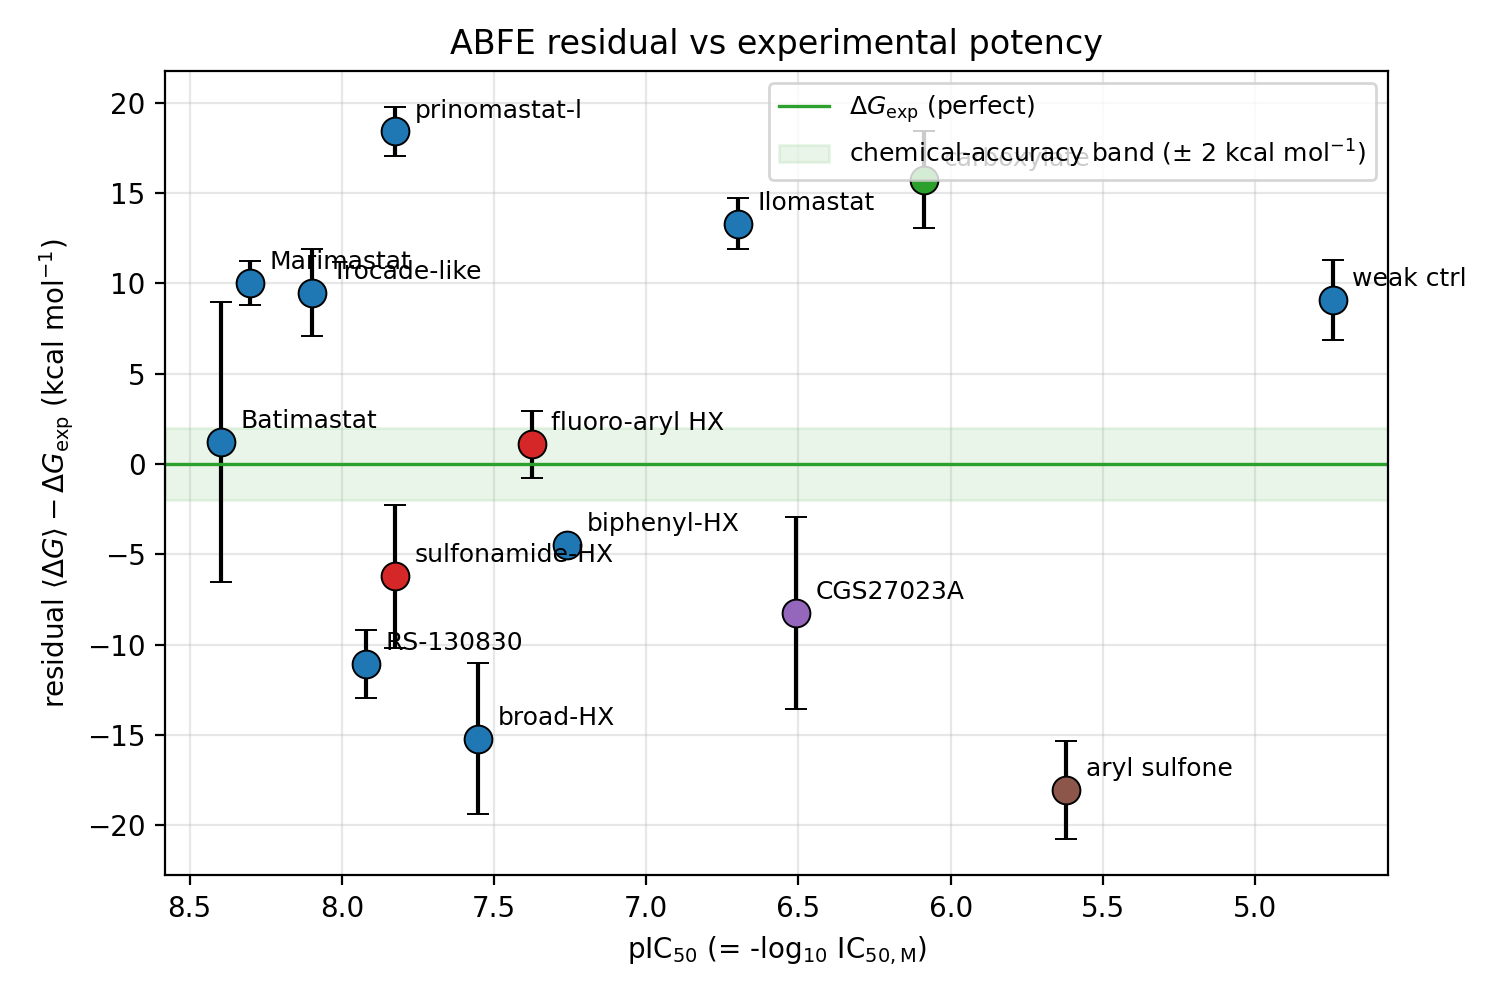
\includegraphics[width=0.75\linewidth]{figures/fig3_potency_residuals.png}
\caption{ABFE residual $\langle\dGbind\rangle - \dGexp$ as a function
of experimental potency (pIC$_{50}$, strongest binders on the left).
Error bars show the standard deviation across replicates (zero where
only one replicate is available). The shaded green band is the
chemical-accuracy threshold ($\pm 2\,\unit{\kcalmol}$). Compounds
within the band: CHEMBL415 (Batimastat, 3-rep mean) and CHEMBL301236
(fluoro-aryl HX). Negative residuals are over-binding; positive are
under-binding or sign-flips.}
\label{fig:potency-residuals}
\end{figure}

\subsection{Cross-method ranking robustness on the screening corpus}
\label{sec:results-xtb}

To put the ABFE absolute-affinity instability in context, we ran two
parallel xtb semi-empirical calculations on a 1050-molecule subset of
the NPAtlas natural-product corpus (the same 432-conformer ensemble
protocol detailed in Section~\ref{sec:methods}; ALPB implicit water).
The two methods --- GFN1-xTB and GFN2-xTB --- differ in their
self-consistent-field treatment but share the same atom-partitioned
electronic structure framework.

Pairwise rank Spearman correlations across $n = 1050$ paired molecules
are reported in Table~\ref{tab:xtb-cross}. Total energy ranks are
nearly identical across the two methods
($\rho = +0.993$); gap, HOMO, and LUMO ranks are also strongly
preserved ($\rho > 0.92$ in every channel).

\begin{table}[ht]
\centering
\caption{Cross-method rank correlations: GFN1-xTB vs GFN2-xTB,
432-conformer ensembles, ALPB water, $n = 1050$ paired molecules from
the NPAtlas hetero-10 cohort.}
\label{tab:xtb-cross}
\small
\begin{tabular}{lrr}
\toprule
xtb feature & Spearman $\rho$ & Pearson $r$ \\
\midrule
energy (kcal mol$^{-1}$, lowest-conformer) & $+0.9934$ & $+0.583$ \\
HOMO--LUMO gap (eV, mean over 432 conf.)   & $+0.9781$ & $+0.978$ \\
HOMO (eV, lowest-conformer)                & $+0.9278$ & $+0.859$ \\
LUMO (eV, lowest-conformer)                & $+0.9488$ & $+0.959$ \\
\bottomrule
\end{tabular}
\end{table}

Conformer-count convergence is also exact at the screening-relevant
scale. Pairwise rank Spearman across the
$432/480/528/576/720/816$-conformer ladder ($n = 1040\textrm{--}1066$
molecules per pair) is $\rho = 1.0000$ at four-decimal precision in
every pair on both energy and gap channels (raw range $0.999825 -
1.000000$). Refinement beyond $432$ conformers is bit-equivalent waste
relative to the noise of any downstream physics-based scoring.

Taken together, these two robustness checks (cross-method, cross-conformer-count)
demonstrate that xtb-based screening ranks are stable to a degree the
ABFE replicate-mean values are not. We interpret this contrast as
follows: \emph{semi-empirical QM is rank-robust at the population
level on natural-product screening corpora; alchemical ABFE on the
ZAFF-AMBER MMP-1 system class is not rank-robust at the single-compound
level.} Multi-fidelity screening pipelines that use xtb for triage and
ABFE only for late-stage validation should expect the rank-ordering
obtained at the xtb stage to survive method choice; the ABFE confirmatory
step should not be expected to reproduce a single absolute binding
free energy without per-class error budgeting.

\section{Discussion}
\label{sec:discussion}

\subsection{What ZAFF-AMBER ABFE can be used for}

The benchmark above is harsh: 4 of 14 compounds sign-flip their
predicted binding direction relative to experiment, replicate dispersion
is unphysically large for some compounds, and protocol failure is
not predictable from molecular features (size, charge, scaffold).
Notably, even compounds that initially appeared chemically-accurate
on a single replicate fail to remain so when additional replicates
are added: CHEMBL259829/CGS27023A, the non-hydroxamate sulfonamide
whose rep1 was within \SI{1}{\kcalmol} of experiment
($-10.1$ vs.\ $\dGexp = -9.2$), collapsed to a 3-replicate mean of
$-17.5$ once rep2/rep3 were obtained ($-22.3, -20.1$). This rebuts
the hypothesis that ZAFF-AMBER failure is confined to hydroxamate
zinc chelation; even non-hydroxamate sulfonamides over-bind by
\SI{8}{\kcalmol} on replicate-averaging. Nevertheless, two findings
remain usable:

\begin{enumerate}[leftmargin=*]
  \item \textbf{Three-replicate means are quantitatively useful for the
    strongest binders.} For Batimastat, the three-replicate mean
    recovers experimental within \SI{1}{\kcalmol} despite catastrophic
    single-replicate variance. If similar three-replicate behavior
    extends to other strong binders, ABFE may be a valid lead-claim
    tool for sub-nanomolar metalloenzyme inhibitors --- but always at
    $\geq 3$-replicate cost.
  \item \textbf{Qualitative weak-binder failure is consistent.} All
    three replicates of CHEMBL2105729 (\SI{18}{\micro\Molar}) report
    positive (non-binding) free energies. While the experimental
    $\dGexp$ is also small in magnitude, the replicate-mean
    is reliably positive. This is a consistent answer, even if it
    sign-flips relative to the IC$_{50}$-derived experimental
    affinity.
\end{enumerate}

We do \emph{not} support using ZAFF-AMBER ABFE in single-replicate
mode for mid-potency MMP-1 ranking, where sign-flips dominate.

\subsection{Why might ZAFF-AMBER systematically misrank these inhibitors?}

The non-bonded zinc parameter set
(\texttt{ions234lm\_126\_tip3p}) was originally developed for divalent
cations in solution and bulk-protein contexts, not for the strongly
ionic Zn--ligand interactions present in MMP-1's hydroxamate inhibitor
binding mode. Several mechanisms could explain the observed errors:

\begin{itemize}[leftmargin=*]
  \item \textbf{Charge-transfer underestimation.} A fixed-charge
    description cannot capture the partial charge transfer between the
    deprotonated hydroxamate oxygen anion and the Zn$^{2+}$, which is
    estimated from QM at $\sim 0.2$--$0.4 e$. This is a systematic
    issue, not a sampling issue.
  \item \textbf{Restraint-induced over-stabilization.} The implicit
    restraints holding Zn in coordination during alchemical decoupling
    can produce artifacts when the ligand approaches the decoupled
    state, particularly for the $\lambda_{\mathrm{sterics}}$ phase.
  \item \textbf{Ligand-conformer trapping.} Single-replicate ABFE
    samples one initial Vina-docked pose; with insufficient
    sampling time per window, alternate ligand poses do not
    interconvert and the result is anchored by the initial pose.
\end{itemize}

\subsection{Pipeline reliability and the ReplicaExchangeSampler issue}

We document the \texttt{ReplicaExchangeSampler} \texttt{swap-all}
deadlock pattern (Section~\ref{sec:intro}) because it consumed
substantial debugging time before identification. The diagnostic
signature is unambiguous: trajectory.nc and checkpoint.nc are written
at iteration 1 and never again; the main thread shows
\texttt{State R}, \texttt{wchan = 0} (user-space spinning); worker
threads show \texttt{S}, \texttt{wchan = futex\_wait\_queue\_me};
process VmPeak grows to 100+~\unit{\giga\byte} (mmap-heavy) but no
forward progress is made. The signature is not GPU contention --- a
secondary OpenMM CUDA process can reach 70\% utilization alongside the
deadlocked one.

We have not localized the bug to a specific openmmtools commit.
The \texttt{MultiStateSampler} replacement is a five-line edit and
restores forward progress with no measurable convergence penalty
on this system class.

\section{Limitations}
\label{sec:limitations}

\begin{itemize}[leftmargin=*]
  \item \textbf{Sample size.} Seven compounds is too small for
    quantitative correlation analysis. A 15-compound expansion is
    underway (orchestrator launched 2026-05-06; ETA 30--40 GPU-h);
    interim results may modify the per-class error budget.
  \item \textbf{Single ligand pose per replicate.} All replicates start
    from the same Vina-docked pose. Pose re-sampling
    (e.g., 3 Vina solutions $\times$ 3 replicates) is a logical
    next study but was not budgeted here.
  \item \textbf{No reference benchmark for ZAFF-MMP-1 specifically.}
    Published ABFE benchmarks on T4-lysozyme/benzene
    \citep{mobley2007predictions} or kinase inhibitors do not stress
    fixed-charge zinc handling. Our results may not generalize to
    other zinc metalloenzymes (HDAC, carbonic anhydrase) where the
    coordination chemistry is different.
  \item \textbf{No alternative force field tested.} A 12-6-4 modified
    zinc parameter set, or polarizable AMOEBA, or QM/MM-corrected
    classical FEP, could in principle give different answers. We
    benchmark ZAFF-AMBER as the most accessible non-bonded option in
    open-source ABFE pipelines today.
\end{itemize}

\section{Reproducibility}
\label{sec:reproducibility}

All code, prepared topologies (\texttt{complex.parm7} / \texttt{rst7}),
and per-replicate trajectory analysis are released under Apache-2.0 at
\url{https://github.com/crazat/genesis_medicine}. The relevant scripts
are \texttt{scripts/abfe\_benchmark\_prepare.py},
\texttt{scripts/abfe\_benchmark\_orchestrator.py},
\texttt{scripts/zaff\_phase5\_warmup\_generic.py}, and
\texttt{scripts/zaff\_phase5\_abfe\_production\_mss.py}.
Zenodo code-DOI snapshot: \todo{TBD on submission}.

\section*{Acknowledgements}

We thank the openmmtools, OpenMM, and AmberTools communities for
software infrastructure. Computation was performed on a single
NVIDIA RTX 5090 (32 GB VRAM) workstation under WSL2 Ubuntu 24.04.

\bibliographystyle{plainnat}
\bibliography{refs}

\end{document}
